\chapter{Utilisation}

Galaxy est un logiciel qui peut être utilisé de trois façon différentes : 

\begin{itemize}
\item en ligne, depuis le site web de ce dernier,
\item sur un "cloud",
\item en local, directement sur son ordinateur.\\
\end{itemize}

La création de sa propre instance de Galaxy sur le "cloud" permet une utilisation de celui-ci similaire à celle en local sans l'inconvénient de la place prise en mémoire sur son ordinateur, toutefois un compte Amazon Web Services est requis.\\

La création du compte est gratuite, cependant un numéro de carte bleue doit être renseigné, en effet il semble que l'utilisation de l'ensemble des fonctionnalitées du "cloud" ai un coût. Nous n'avons donc pas pu tester Galaxy sur le "cloud".\\

\section{En ligne}

L'utilisation en ligne de Galaxy est le moyen le plus rapide et le plus accessible : en effet il suffit de se rendre sur le site de ce dernier pour pouvoir y avoir directement accès. Si une utilisation sommaire ne nécessite pas la création d'un compte, il est fortement recommandé d'en créer un (gratuitement) pour avoir accès à plus de fonctionnalité. Posséder un compte sur Galaxy permet :\\

\begin{itemize}
\item d'avoir accès aux données et aux outils d'analyse depuis n'importe quel ordinateur connecté à Internet,
\item augmenter les données et les travaux simultanés,
\item sauvegarder un historique de compte sur une base systémique,
\item d'avoir la capacité de nommer, sauvegarder, partager et publier des objets de Galaxy : des historiques, des workflows, des ensembles de données, des pages.
\item de télécharger via le FTP de plus grands ensembles de données.\\
\end{itemize}

Galaxy dispose de nombreux outils (plus de 35 différents), heureusement lorsque l'on sélectionne l'un d'entre eux une petite fenêtre explicative nous renseigne directement sur ce qu'il fait, le format de données qu'il accepte et un exemple est également proposé (Fig. 6).\\


\begin{figure}[!h]
 \centering
\fbox{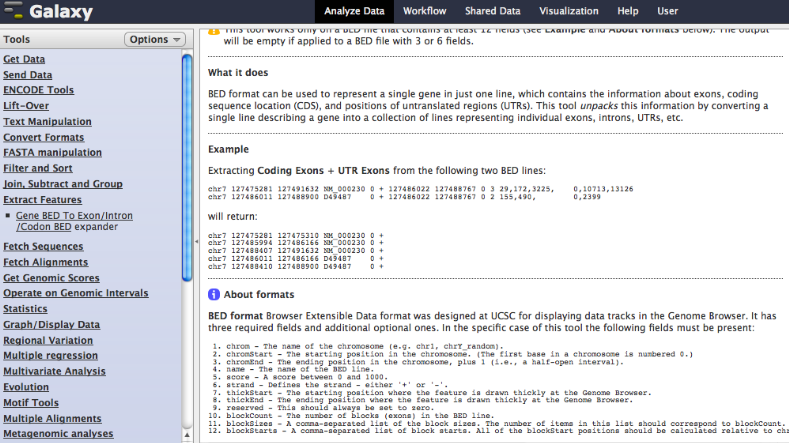
\includegraphics[scale=0.5]{Images/exinfo.png}}
\caption{Page d'aide d'un des outils de Galaxy.}
\end{figure}

Un wiki dédié à Galaxy est disponible sur son site, plusieurs sections différentes permettent d'en apprendre plus sur les données que peut utiliser Galaxy et les outils qu'il propose. De plus de nombreuse vidéos "tutoriel" sont disponibles, ainsi un exercice nommé Galaxy 101 fait office de "tutoriel" de départ et permet de se familiarisé avec le logiciel et quelques unes de ces fonctionnalitées. Une vidéo "tutoriel" est disponible pour chaque outil intégré à Galaxy (Fig. 7).

\begin{figure}[!h]
 \centering
\fbox{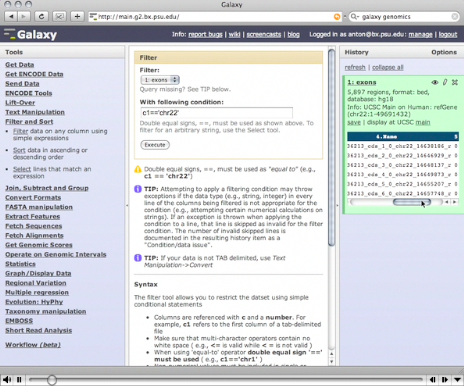
\includegraphics[scale=0.5]{Images/tuto.png}}
\caption{Vidéo "tutoriel" de Galaxy.}
\end{figure}

\section{En local}

En plus de proposer une utilisation via internet, il est possible d'installer Galaxy sur un ordinateur. L'utilisateur peut ainsi profiter de toutes les fonctionnalités de Galaxy et même les personnaliser en vue d'une utilisation spécifique\footnote{Le tutorial officiel de l'installation locale est disponnible à l'adresse suivante :\\ http://wiki.g2.bx.psu.edu/Admin/Get\%20Galaxy}.\\

Par rapport à l'utilisation en ligne, le local présente plusieurs avantages :
\begin{itemize}
\item modifier les paramètres des plug-ins déjà implémentés,
\item ajouter ses propres plug-ins,
\item augmenter la vitesse d'analyse,
\item conserver des données sensibles.\\
\end{itemize}

L'installation est très simple et se déroule en deux étapes :
\begin{enumerate}
\item téléchargement du code source,
\item exécution du serveur local.
\end{enumerate}

\subsection{Téléchargement du code source}

La dernière version stable de Galaxy est toujours disponible depuis un répertoire Mercurial\footnote{http://mercurial.selenic.com/} hébergé sous Bitbucket\footnote{https://bitbucket.org/}. Il existe deux façons de récupérer le code source : en utilisant les outils proposés par Bitbucket ou en utilisant Mercurial.

\subsection*{Bitbucket}

Bitbucket est un site d'hébergement pour les systèmes de contrôles de versions Git\footnote{http://git-scm.com/} et Mercurial. Il offre aussi de nombreux outils tels que : Issue tracker, Wiki, Basecamp, Flowdock, Twitter, etc ...\\

Ses principaux avantages sont la facilité d'utilisation, sa gratuité (sous réserve d'avoir moins de cinq collaborateurs sur tous les répertoires privés) ainsi que les aides proposées (nombreux tutoriaux, large communauté, Google group, I.R.C, etc ...).\\

Le téléchargement de Galaxy est simple : il suffit, dans l'onglet \textit{Source} (Fig. 8), de cliquer sur \textit{get source} et de sélectionner le mode de compression désiré (Fig. 9).

\begin{figure}[!h]
 \centering
\fbox{
\includegraphics[scale=0.7]{Images/Bitbucket1.png}}
\caption{Onglets disponibles (Bitbucket).}
\end{figure}
\begin{figure}[!h]
 \centering
\fbox{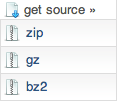
\includegraphics[scale=0.7]{Images/Bitbucket2.png}}
\caption{Téléchargement du code source (Bitbucket).}
\end{figure}

Ce mode de récupération est très simple mais présente un gros inconvénient : il sera impossible de mettre Galaxy à jour de cette façon.

\subsection*{Mercurial}

Mercurial est un outil de gestion de versions développé depuis 2005 sous licence GNU GPL. Principalement écrit en Python et utilisable en ligne de commande, Mercurial n'en est pas moins rapide, robuste et facile d'utilisation.\\

Toutes les commandes de Mercurial commencent par \textit{hg}, formule chimique du mercure.\\

La copie du répertoire distant tient en quelques commandes : 
\lstset{language=sh}
\begin{lstlisting} [morekeywords={mkdir,hg}]
mkdir Galaxy
cd Galaxy
hg clone https://bitbucket.org/galaxy/galaxy-dist/
 \end{lstlisting} 

Le clonage prend un certain temps. Mercurial doit en effet analyser les nouveautés du répertoire distant et télécharger les fichiers un par un. Le dossier final contient $\sim$8000 fichiers pour une taille totale d'environ 700 Mo.\\

L'intérêt d'utiliser Mercurial pour récupérer le code source est de pouvoir mettre ce code à jour, contrairement à Bitbucket.\\
La mise à jour utilise le système de modification distance de Mercurial. Elle tient donc en deux commandes\footnote{A exécuter dans le répertoire local de Galaxy} : 
\lstset{language=sh}
\begin{lstlisting} [morekeywords={hg}]
hg incoming
hg pull -u
 \end{lstlisting} 
 La première commande indique si des modifications ont été apportées. Si elle renvoie \textit{no changes found}, la version locale est à jour. Dans le cas contraire, elle renvoie une liste de \textit{changeset} (Fig. 10). La seconde commande peut être exécutée si au moins \textit{changset} est indiqué.

\begin{figure}[!h]
 \centering

\fbox{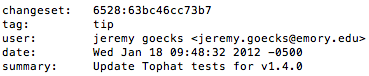
\includegraphics[scale=0.7]{Images/Changeset.png}}
\caption{Exemple de \textit{changeset} (Mercurial).}
\end{figure}

\subsection{Exécution du serveur local}

Galaxy fonctionne sur la base d'un serveur local. Cela consiste à ouvrir un serveur fictif sur l'ordinateur de l'utilisateur et à se servir de l'interface proposée par un navigateur web pour accéder aux services proposés par le serveur.\\

Ce logiciel étant principalement écrit en Python, il est officiellement compatible avec les versions 2.5, 2.6 et 2.7 de l'interpréteur Python par défaut. La version par défaut est donnée en en-tête de l'interpréteur  
(Fig. 11).

 \begin{figure}[!h]
 \centering
\fbox{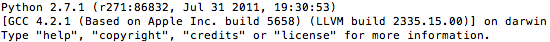
\includegraphics[scale=0.7]{Images/Python.png}}
\caption{Version de l'interpréteur Python.}
\end{figure}

Pour lancer le serveur local de Galaxy, il suffit d'exécuter le script \textit{run.sh} : 
\lstset{language=sh}
\begin{lstlisting} [morekeywords={sudo}]
sh run.sh # commande de base
sudo run.sh # commande administrateur
 \end{lstlisting} 
 
 La commande "de base" suffit à démarrer le serveur. Il est toutefois conseillé d'utiliser la commande administrateur car certaines opérations \footnote{Notamment l'écriture sur disque dur.} nécessitent des droits d'administrateur.\\
 
 Le serveur charge tous les fichiers requis, configure ses variables et démarre sur une adresse indiquée sur la dernière ligne du terminal (Fig. 12).
 
 \begin{figure}[!h]
 \centering
\fbox{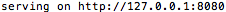
\includegraphics[scale=0.7]{Images/Adresselocale.png}}
\caption{Adresse du serveur de Galaxy.}
\end{figure}

Pour stopper le serveur, il suffit d'utiliser \textit{ctrl+z} dans le terminal qui le gère.\\

Il est possible que le port utilisé par Galaxy soit déjà en utilisation. Dans ce cas, le démarrage du serveur échoue et renvoie une erreur \textit{adress already in use} (Fig. 13). Seul un redémarrage de l'ordinateur peut réinitialiser le port.

 \begin{figure}[!h]
 \centering
\fbox{
\includegraphics[scale=0.7]{Images/Socketerror.png}}
\caption{Erreur d'adressage de port.}
\end{figure}
Une fois le serveur démarré, son accès est possible depuis un navigateur web quelconque (Fig. 14). L'adresse URL à indiquer est l'adresse donnée sur la dernière ligne du terminal.

 \begin{figure}[!h]
 \centering
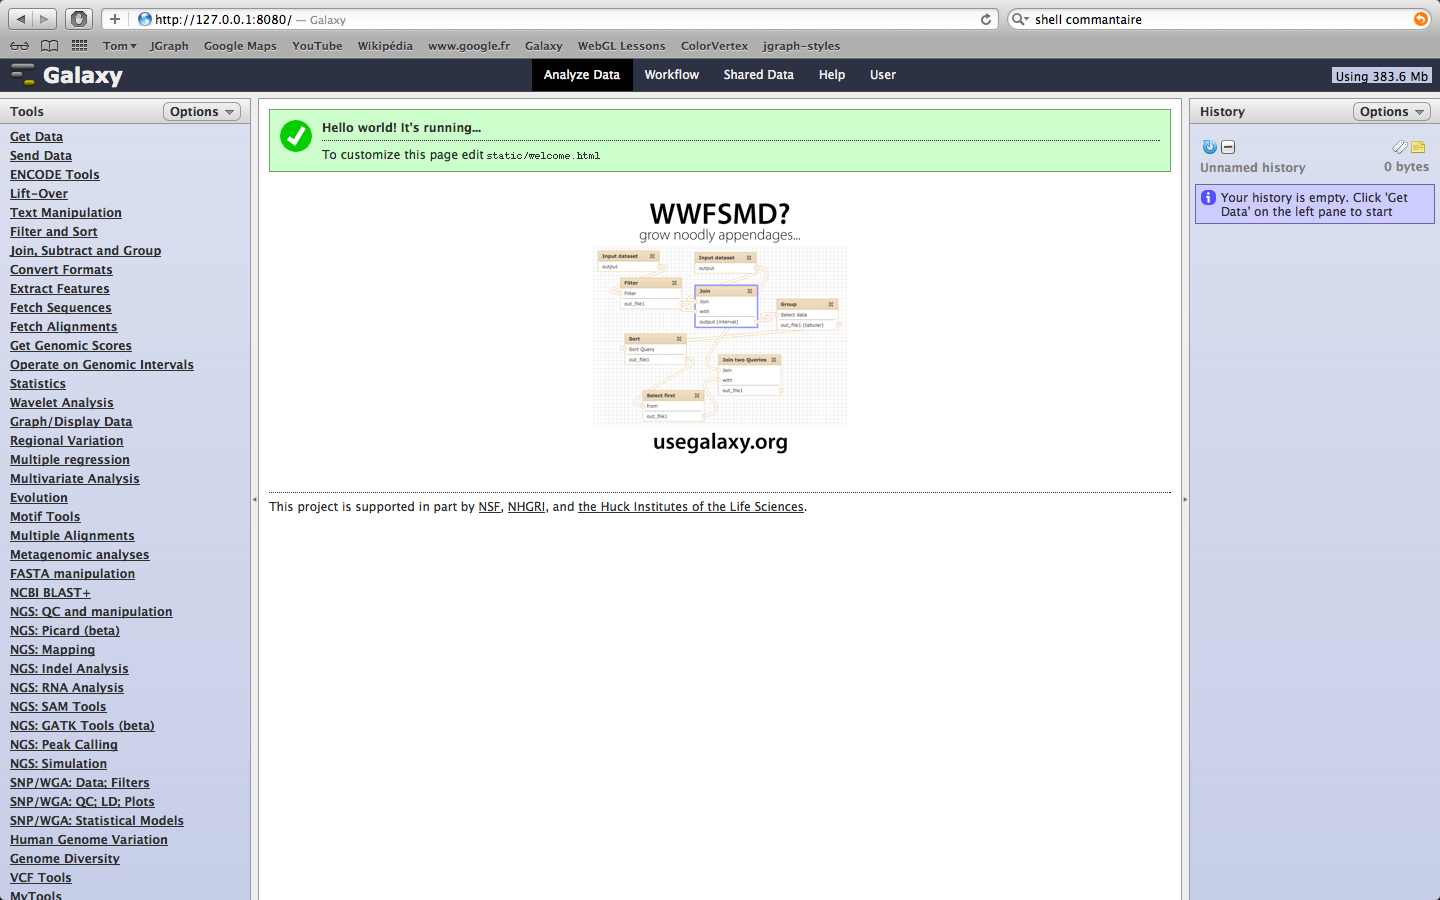
\includegraphics[scale=0.35]{Images/Galaxylocal.png}
\caption{Galaxy en usage local.}
\end{figure}